\section{Unstable manifolds and shadowing}
\label{sect:shadow}

Unstable manifolds of the three \eqva\ and the two \reqva,
and their connecting orbits in the full
\statesp\ have been discussed in detail in\rf{SCD07}.
With the advance in the technique of
symmetry reduction, we have a better picture of the in-slice \statesp.
Moreover, \rpo s become periodic in the slice, which helps us
organize the pre/relative \po s in our database.
In this section, we will discuss the unstable manifolds of
(relative) \eqva\ and show shadowing incidences of different orbits.

\subsection{\On{2} symmetry reduction}
\label{sect:ksO2}

\refSect{sect:kssym} introduces the 1st mode slice to reduce \SOn{2}
in the one\dmn\ \KSe. Here, we go one step further, \ie, quotienting
out reflection symmetry in the 1st mode slice.
Different from the invariant polynomial approach used by
N. B. Budanur\rf{BudanurThesis, BudCvi15}, we turn to the fundamental
domain.

In \refsect{sect:kssym}, the 1st mode slice \refeq{eq:ksslice}
is defined as the half hyperplane $c_1=0$, \ie, the imaginary
part of the 1st mode vanishes. Here, when reducing reflection in the slice,
we find it is more convenient to define the slice as
\begin{equation}
  \label{eq:ksslice2}
  b_1 = 0,\, c_1 > 0 \,,
\end{equation}
namely, we let the real part of the 1st mode vanish.
Literature\rf{BudCvi14, DCTSCD14} all chooses \refeq{eq:ksslice}.
That is why we insist on using \refeq{eq:ksslice} to define the 1st mode
slice in other chapters of this thesis.
Thus conversion \refeq{eq:ksslice2}
is only used in this section. The benefit of using \refeq{eq:ksslice2}
instead of \refeq{eq:ksslice} in this section
is that the reflection axis is parallel
to the slice \refeq{eq:ksslice2} such that the reflection rule does
not change from the full \statesp\ to the slice.
%%% example start %%%
\exampl{
  Reflection rule is invariant under \SOn{2} reduction
  by \refeq{eq:ksslice2} }{
  \label{exam:ksreflect}
  Suppose two states $\ssp_1$ and $\ssp_2$ in
  the full \statesp\
  are related to each other by reflection, $\ssp_2 = R\ssp_1$.
  Let $\sspRed_1$ and $\sspRed_2$ be their reduced states in the slice
  \refeq{eq:ksslice2}.
  If the 1st Fourier mode of $\ssp_1$ is $(b_1 + ic_1)$, then
  the 1st Fourier mode of  $\ssp_2$ is $(-b_1 + ic_1)$.
  \begin{figure}[ht]
    \centering
    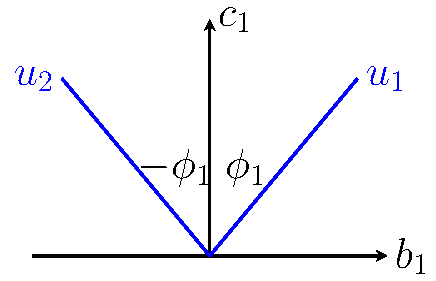
\includegraphics[width=0.4\textwidth]{sliceAngle}
    \caption{Illustration of the phase relation in \refexam{exam:ksreflect}.}
    \label{fig:sliceAngle}
  \end{figure}
  So if $\LieEl(\gSpace_1)$ transforms $\ssp_1$ onto the positive
  imaginary axis in $(b_1, c_1)$ plane, that is,
  $\sspRed_1 = \LieEl(\gSpace_1) \ssp_1$, then
  $\sspRed_2 = \LieEl(-\gSpace_1) \ssp_2$ as shown in
  \reffig{fig:sliceAngle}.
  Therefore,
  \[
    \sspRed_2 = \LieEl(-\gSpace_1) R\ssp_1
    = R\LieEl(\gSpace_1) \ssp_1
    = R \sspRed_1
    \,.
  \]
  Here we have used the anti-commuting relation
  $\LieEl(-\gSpace) R = R\LieEl(\gSpace)$. So we see that
  the choice of slice \refeq{eq:ksslice2} keeps the reflection rule
  unchanged.
}
%%% example end %%%

The reflection operator is $R=\diag(-1,\, 1, \, -1, \, 1,\cdots)$.
Since $\hat{b}_1 =0$ in the slice, thus $\hat{b}_k$ with $k>1$ changes sign
after reflection. We define the fundamental domain in the slice as
\begin{equation}
  \label{eq:fundDomain}
  \hat{b}_2 > 0
  \,.
\end{equation}
Whenever an in-slice orbit leaves the fundamental domain, we transform
it back by reflection. With the sacrifice of allowing discontinuity,
we quotient out \On{2} symmetry in the one\dmn\ \KSe.

\subsection{Unstable manifold of \EQV{2} }

There are three \eqva\  \EQV{1}, \EQV{2} and \EQV{3} and two
\reqva\ \REQV{1}{} and \REQV{2}{} in this system.
$E_2$ and $E_3$ are symmetric under shifts by $L/2$ and
$L/3$ respectively as shown in \reffig{fig:kseq}.
As shown in\rf{SCD07}, one branch of the unstable manifold of
\EQV{1} and the unstable manifold of \EQV{3} terminate at \EQV{2}
or its symmetry-equivalent counterparts in the full \statesp.
Also, the unstable manifold of \EQV{2} is a set of
homoclinic orbits of itself.
Therefore, we believe that
\EQV{2} has a large influence on the geometrical structure
of the in-slice \statesp.

\refFig{fig:E2Wu} shows the unstable manifold of
\EQV{2} and several pre/relative \po s in the fundamental
domain projected into
some Fourier mode subspace. Since \EQV{2} and \EQV{3}
are in the {\sliceBord}, their \SOn{2} symmetry can not be
quotiented out by the 1st mode slice.
The blue and green straight lines are the group orbits of
\EQV{2} and \EQV{3} in the slice respectively. These
two lines depict the slice border in this three\dmn\ subspace.
Note, this does not mean that the unstable manifold of
\EQV{2} should also live in the slice. Actually, \EQV{2}
has one pair of unstable complex conjugate stability
eigenvectors, which
do have nonzero first Fourier mode components. Hence,
the corresponding unstable manifolds have unique locations,
determined by the first Fourier mode phase of this pair of
eigenvectors, in the symmetry reduced \statesp.

\begin{figure}[!ht]
  \centering
  (a)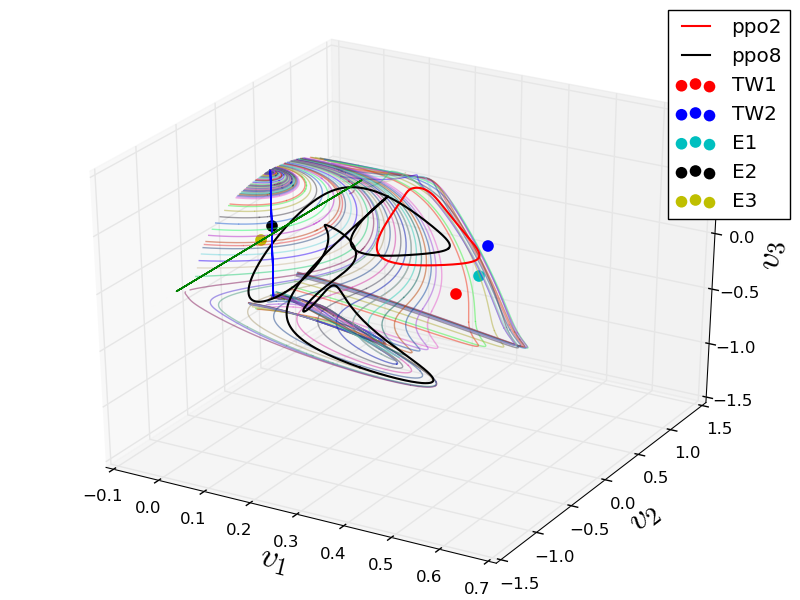
\includegraphics[width=0.8\textwidth]{ppo8}
  (b)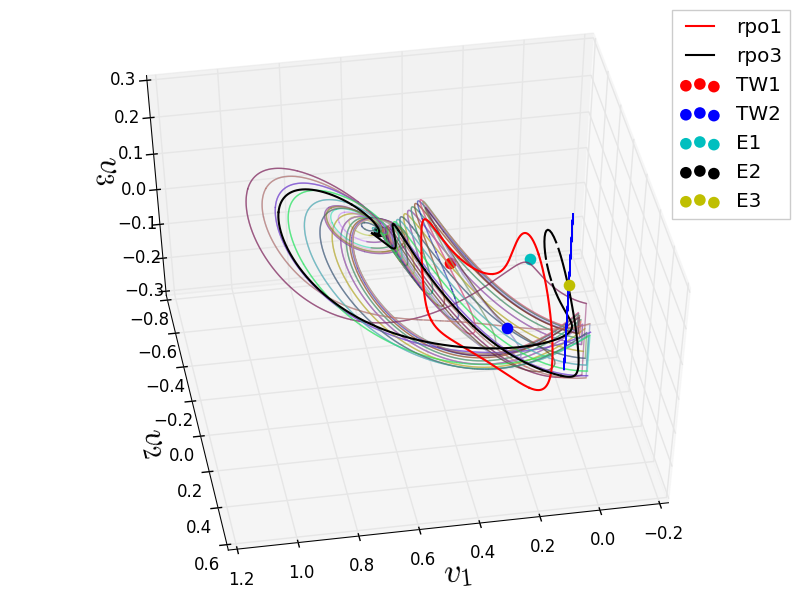
\includegraphics[width=0.8\textwidth]{rpo3}
  \caption[The unstable manifold of \EQV{2}.]{
    The unstable manifold of \EQV{2} in the fundamental domain in the
    slice.
    The dense set of thin curves is the unstable
    manifold of \EQV{2}.
    The blue and green straight lines are the group orbits of
    \EQV{2} and \EQV{3} respectively.
    \texttt{ppo2} is \PPO{14.33} in \reffig{fig:kspoT100}.
    \texttt{rpo1} is \RPO{16.31}.
    \texttt{ppo8} is \PPO{41.08}. \texttt{rpo3} is \RPO{33.50}.
    Projection axes are the imaginary parts of the first 3 Fourier modes
    $[v_1, v_2, v_3] = [\hat{c}_1, \hat{c}_3, \hat{c}_2]$.
    This set is invariant under reflection.
  }
  \label{fig:E2Wu}
\end{figure}

There are a few interesting observations in \reffig{fig:E2Wu}.
First, the pre/relative \po s look continuous,
but in fact, they are discontinuous in the fundamental domain.
We choose the three\dmn\ subspace to be $(\hat{c}_1, \hat{c}_3, \hat{c}_2)$
which is invariant under reflection. Thus reflection has no effect
on this specific projection. Second,
the unstable manifold of \EQV{2} is discontinuous.
Whenever it crosses the slice border, there is a phase jump by $\pi$,
which causes $\hat{c}_3$ to change sign. Third, we can see that both
\texttt{ppo8} (\PPO{41.08}) and \texttt{rpo3} (\RPO{33.50}) shadow
the unstable manifold of \EQV{2} for a certain period of time.
Actually, there are plenty of
pre/relative \po s in our database that shadow
the unstable manifold of \EQV{2}.
In this sense, \EQV{2} plays a substantial role in shaping  the dynamics.

\subsection{Shadowing among orbits}

\begin{figure}[!ht]
  \centering
  (a)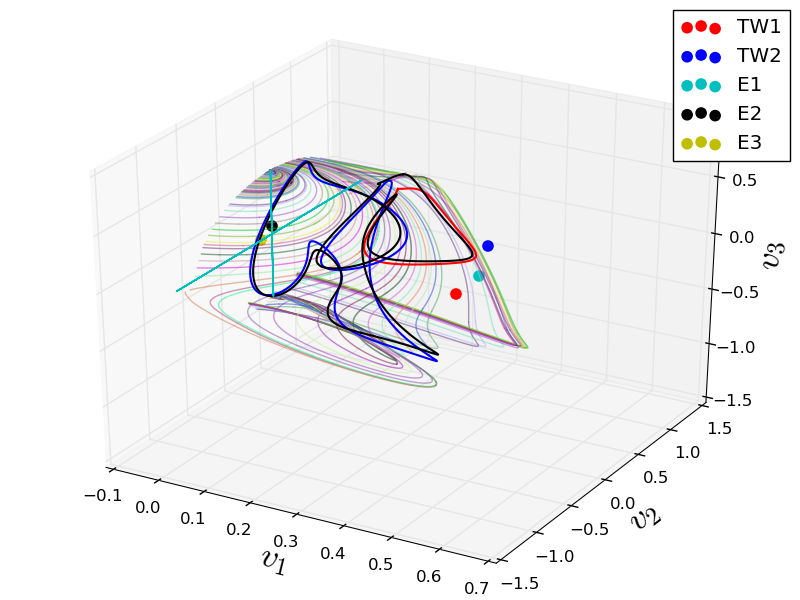
\includegraphics[width=0.8\textwidth]{rpo1rpo5rpo22Im}
  (b)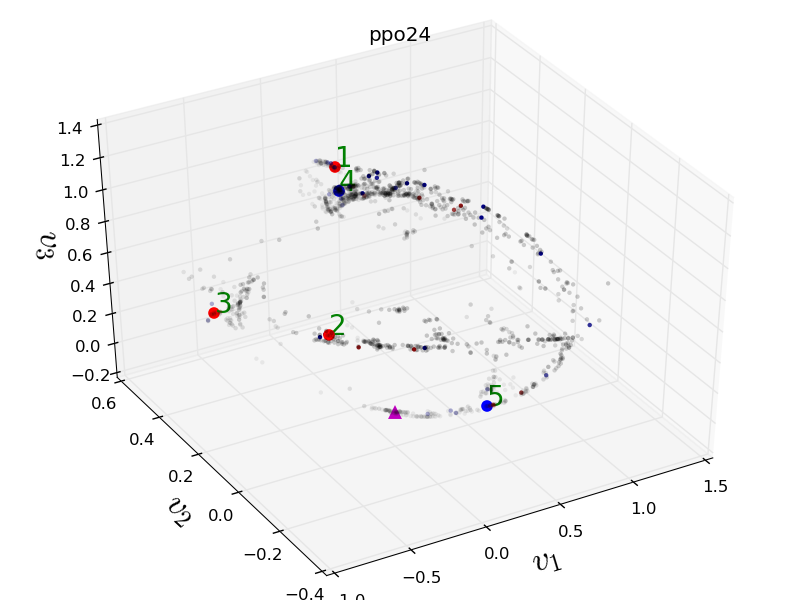
\includegraphics[width=0.8\textwidth]{ppo24}
  \caption[Shadowing among pre/relative \po s]{
    Shadowing among pre/relative \po s in the fundamental domain.
    The dense set of thin curves is the unstable
    manifold of \EQV{2}. The two  straight lines are the group orbits of
    \EQV{2} and \EQV{3} respectively.
    Projection axes are the imaginary parts of the first 3 Fourier modes
    $[v_1, v_2, v_3] = [\hat{c}_1, \hat{c}_3, \hat{c}_2]$.
    This set is invariant under reflection.
    (a)
    The three \rpo s are (red) \RPO{16.31}, (blue) \RPO{35.97}
    and (black) \RPO{57.59}.
    (b)
    The red pre\po\ is \texttt{ppo2} (\PPO{14.33}).
    The black pre\po\ is \texttt{ppo24} (\PPO{57.67}).
  }
  \label{fig:shadow}
\end{figure}

In \reffig{fig:E2Wu}, we see that \texttt{ppo2} (\PPO{14.33})
is quite similar to \texttt{rpo1} (\RPO{16.31}). Actually,
these two orbits shadow each other and have similar
periods. There are a lot of other shadowing incidences between
different pre/relative \po s. For example, in
\reffig{fig:shadow}(a), \RPO{57.59} shadows \RPO{16.31} and
\RPO{35.97} closely. The period of this longer orbit is close to the
sum of the periods of the two shorter orbits. In \reffig{fig:shadow}(b),
\PPO{57.67} shadows \PPO{14.33} for a certain period of time.
Shadowing helps us classify all the
pre/relative \po s and helps build the symbolic
dynamics of this system. This is important for the \Fd\
\refeq{eq:sd} to converge quickly when it is expanded by only a few short
orbits\rf{DasBuch}.

On the other hand, pre\po s and \rpo s frequently show up in pairs
in the one\dmn\ \KSe. For instance,
\RPO{57.59} in \reffig{fig:shadow}(a) and \PPO{57.67} in
\reffig{fig:shadow}(b) are such a pair.
N. B. Budanur and P. Cvitanovi\'c\rf{BudCvi15} believe that this
phenomenon comes from symmetry-breaking bifurcation as
the domain size $L$ is varied.
